%éléments communalisés
\pgfdeclareimage{case}{01-EtudeAeronefs/img/instruments/alt/alt_case.pdf}

\pgfdeclareimage{asiFace}{01-EtudeAeronefs/img/instruments/asi/asi_face.pdf}
\pgfdeclareimage{asiHand}{01-EtudeAeronefs/img/instruments/asi/asi_hand.pdf}
\pgfdeclareimage{asiCase}{01-EtudeAeronefs/img/instruments/asi/asi_case.pdf}

\pgfdeclareimage{altCase}{01-EtudeAeronefs/img/instruments/alt/alt_case.pdf}
\pgfdeclareimage{altFace1}{01-EtudeAeronefs/img/instruments/alt/alt_face_1.pdf}
\pgfdeclareimage{altFace2}{01-EtudeAeronefs/img/instruments/alt/alt_face_2.pdf}
\pgfdeclareimage{altFace3}{01-EtudeAeronefs/img/instruments/alt/alt_face_3.pdf}
\pgfdeclareimage{altHand1}{01-EtudeAeronefs/img/instruments/alt/alt_hand_1.pdf}
\pgfdeclareimage{altHand2}{01-EtudeAeronefs/img/instruments/alt/alt_hand_2.pdf}

\pgfdeclareimage{aiCase}{01-EtudeAeronefs/img/instruments/ai/ai_case.pdf}
\pgfdeclareimage{aiFace}{01-EtudeAeronefs/img/instruments/ai/ai_face.pdf}
\pgfdeclareimage{aiRing}{01-EtudeAeronefs/img/instruments/ai/ai_ring.pdf}
\pgfdeclareimage{aiBack}{01-EtudeAeronefs/img/instruments/ai/ai_back.pdf}

\pgfdeclareimage{hiCase}{01-EtudeAeronefs/img/instruments/hi/hi_case.pdf}
\pgfdeclareimage{hiFace}{01-EtudeAeronefs/img/instruments/hi/hi_face.pdf}

\pgfdeclareimage{tcCase}{01-EtudeAeronefs/img/instruments/tc/tc_case.pdf}
\pgfdeclareimage{tcFace1}{01-EtudeAeronefs/img/instruments/tc/tc_face_1.pdf}
\pgfdeclareimage{tcFace2}{01-EtudeAeronefs/img/instruments/tc/tc_face_2.pdf}
\pgfdeclareimage{tcBall}{01-EtudeAeronefs/img/instruments/tc/tc_ball.pdf}
\pgfdeclareimage{tcBack}{01-EtudeAeronefs/img/instruments/tc/tc_back.pdf}
\pgfdeclareimage{tcMark}{01-EtudeAeronefs/img/instruments/tc/tc_mark.pdf}

\pgfdeclareimage{vsiCase}{01-EtudeAeronefs/img/instruments/vsi/vsi_case.pdf}
\pgfdeclareimage{vsiHand}{01-EtudeAeronefs/img/instruments/vsi/vsi_hand.pdf}
\pgfdeclareimage{vsiFace}{01-EtudeAeronefs/img/instruments/vsi/vsi_face.pdf}

\pgfdeclareimage{ilsCase}{01-EtudeAeronefs/img/instruments/ils/ils_case.pdf}
\pgfdeclareimage{ilsCaseFixed}{01-EtudeAeronefs/img/instruments/ils/ils_case_fixed.pdf}
\pgfdeclareimage{ilsFace}{01-EtudeAeronefs/img/instruments/ils/ils_face.pdf}
\pgfdeclareimage{ilsFlagGs}{01-EtudeAeronefs/img/instruments/ils/ils_flag_gs.pdf}
\pgfdeclareimage{ilsFlagNav}{01-EtudeAeronefs/img/instruments/ils/ils_flag_nav.pdf}
\pgfdeclareimage{ilsHandGs}{01-EtudeAeronefs/img/instruments/ils/ils_hand_gs.pdf}
\pgfdeclareimage{ilsHanvNav}{01-EtudeAeronefs/img/instruments/ils/ils_hand_nav.pdf}

%altimètre
%   -paramètre 1 : altitude en pieds
%   -paramètre 2 : calage en pouces de mercure
\def\alti#1#2{
	\fill[transparent] (0,0) circle (3) ;
	\node[rotate=(#2-28.0)*100] {\pgfbox[center,center]{\pgfuseimage{altFace1}}};
	\node {\pgfbox[center,center]{\pgfuseimage{altFace2}}};
  	\node[rotate=-{(Mod(#1/10,10000))*(36/1000)}] {\pgfbox[center,center]{\pgfuseimage{altFace3}}};
  	\node[rotate=-{(Mod(#1,1000))*(360/1000)}] {\pgfbox[center,center]{\pgfuseimage{altHand2}}};
    	\node[rotate=-{(Mod(#1,10000))*(360/10000)}] {\pgfbox[center,center]{\pgfuseimage{altHand1}}};
    	%\node {\pgfbox[center,center]{\pgfuseimage{altCase}}};
	\node {\pgfbox[center,center]{\pgfuseimage{case}}};
}

%consevateur de cap
%   -paramètre 1 : cap en degrés
\def\conservateurCap#1{
	\fill[transparent] (0,0) circle (3) ;
  	\node[rotate=#1] {\pgfbox[center,center]{\pgfuseimage{hiFace}}};
    	\node {\pgfbox[center,center]{\pgfuseimage{hiCase}}};
}

%ILS
%   -paramètre 1 : QDM en degrés
%   -paramètre 2 : décallage horizontal
%   -paramètre 3 : décallage vertical
\pgfkeys{
    /ilsparam/.is family,
    /ilsparam,
    qdm/.store in = \ilsQdm,
    ecartLoc/.store in = \ilsEcartLoc,
    ecartGlide/.store in = \ilsEcartGlide,
    afficherFlagNav/.store in = \ilsAfficherFlagNav,
    afficherFlagGs/.store in = \ilsAfficherFlagGs,
    qdm = 0,
    ecartLoc = 0,
    ecartGlide = 0,
    afficherFlagNav = false,
    afficherFlagGs = false,
}
\newcommand{\ils}[1]{
    \pgfkeys{/ilsparam, #1}
%\def\ils#1#2#3{
	\fill[transparent] (0,0) circle (3) ;
		\node {\pgfbox[center,center]{\pgfuseimage{ilsCaseFixed}}};
		\ifthenelse{\equal{\ilsAfficherFlagGs}{true}}{
			\node {\pgfbox[center,center]{\pgfuseimage{ilsFlagGs}}};
		}
		\ifthenelse{\equal{\ilsAfficherFlagNav}{true}}{
			\node {\pgfbox[center,center]{\pgfuseimage{ilsFlagNav}}};
		}
		\node[yshift=\ilsEcartGlide*31.75] {\pgfbox[center,center]{\pgfuseimage{ilsHandGs}}};
		\node[xshift=\ilsEcartLoc*31.75] {\pgfbox[center,center]{\pgfuseimage{ilsHanvNav}}};
		\node[rotate=\ilsQdm] {\pgfbox[center,center]{\pgfuseimage{ilsFace}}};
    	\node {\pgfbox[center,center]{\pgfuseimage{ilsCase}}};
}

%variomètre
%   -paramètre 1 : taux de descente
\def\vario#1{
	\fill[transparent] (0,0) circle (3) ;
  	\node {\pgfbox[center,center]{\pgfuseimage{vsiFace}}};
   	\node[rotate=-(#1/2000)*172] {\pgfbox[center,center]{\pgfuseimage{vsiHand}}};
    	%\node {\pgfbox[center,center]{\pgfuseimage{vsiCase}}};
	\node {\pgfbox[center,center]{\pgfuseimage{case}}};
}

%horizon
%   -paramètre 1 : roulis
%   -parametre 2 : tangage 
\def\horizon#1#2{
	\fill[transparent] (0,0) circle (3) ;
	\node {\pgfbox[center,center]{\pgfuseimage{aiBack}}};
  	\node[rotate=#1,yshift=-#2*1.25] {\pgfbox[center,center]{\pgfuseimage{aiFace}}};
    	\node[rotate=#1] {\pgfbox[center,center]{\pgfuseimage{aiRing}}};
    	\node {\pgfbox[center,center]{\pgfuseimage{aiCase}}};
}

%indicateur de virage
%   -paramètre 1 : taux virage [-1;1] 
%   -parametre 2 : postion bille [-1;1] 
\def\indicateurVirage#1#2{
	\fill[transparent] (0,0) circle (3) ;
  	\node {\pgfbox[center,center]{\pgfuseimage{tcBack}}};
    	\node {\pgfbox[center,center]{\pgfuseimage{tcFace1}}};
    	\node {\pgfbox[center,center]{\pgfuseimage{tcFace2}}};
    	%\node[xshift=#2*35,yshift=#2*4] {\pgfbox[center,center]{\pgfuseimage{tcBall}}};
	\node[rotate around={#2*15:(0,3.7)}] {\pgfbox[center,center]{\pgfuseimage{tcBall}}};
    	\node[rotate=#1*20] {\pgfbox[center,center]{\pgfuseimage{tcMark}}};
    	%\node {\pgfbox[center,center]{\pgfuseimage{tcCase}}};
	\node {\pgfbox[center,center]{\pgfuseimage{case}}};
}

%badin
%   -paramètre 1 : vitesse [0;200] 
\def\badin#1{
	\fill[transparent] (0,0) circle (3) ;
  	\node {\pgfbox[center,center]{\pgfuseimage{asiFace}}};
    	
	%0 kts : 0°
	%40 kts : 36°
	%70 kts : 90°
	%130 kts : 210°
	%160 kts : 264°
	%200 kts : 312°

	%	Vitesse	Position aiguille	Angle/10 kts
	%	0		0,00°	
	%	40		36,00°		NA
	%	50		54,00°		-18°
	%	60		72,00°		-18°
	%	70		90,00°		-18°
	%	80		110,00°		-20°
	%	90		130,00°		-20°
	%	100		150,00°		-20°
	%	110		170,00°		-20°
	%	120		190,00°		-20°
	%	130		210,00°		-20°
	%	140		228,00°		-18°
	%	150		246,00°		-18°
	%	160		264,00°		-18°
	%	200		312,00°		-12°

	%Entre 0 et 40 kts
	\ifnum#1<41
	\node[rotate=-(((#1)/(40))*(36))] {\pgfbox[center,center]{\pgfuseimage{asiHand}}};
	\fi 
	%Entre 40 et 70 kts
	\ifnum#1>40 \ifnum#1<71
	\node[rotate=-(((#1-40)/(70-40))*(90-36))-36] {\pgfbox[center,center]{\pgfuseimage{asiHand}}};
	\fi \fi
	%Entre 71 et 130 kts
	\ifnum#1>70 \ifnum#1<131
	\node[rotate=-(((#1-70)/(130-70))*(210-90))-90] {\pgfbox[center,center]{\pgfuseimage{asiHand}}};
	\fi \fi
	%Entre 130 et 160 kts
	\ifnum#1>130 \ifnum#1<161
	\node[rotate=-(((#1-130)/(160-130))*(264-210))-210] {\pgfbox[center,center]{\pgfuseimage{asiHand}}};
	\fi \fi
	%Entre 160 et 200 kts
	\ifnum#1>160
	\node[rotate=-(((#1-160)/(200-160))*(312-264))-264] {\pgfbox[center,center]{\pgfuseimage{asiHand}}};
	\fi

    	%\node {\pgfbox[center,center]{\pgfuseimage{asiCase}}};
	\node {\pgfbox[center,center]{\pgfuseimage{case}}};
}

% Définir les clés pour les paramètres
\pgfkeys{
    /tdb/.is family,
    /tdb,
    vitesse/.store in = \tdbVitesse,
    altitude/.store in = \tdbAltitude,
    calageAltitude/.store in = \tdbCalageAltitude,
    vz/.store in = \tdbVz,
    cap/.store in = \tdbCap,
    assiette/.store in = \tdbAssiette,
    inclinaison/.store in = \tdbInclinaison,
    derapage/.store in = \tdbDerapage,
    virage/.store in = \tdbVirage,
    afficherT/.store in = \tdbAfficherT,
    vitesse = 0,
    altitude = 0,
    vz = 0,
    cap = 0,
    assiette = 0,
    inclinaison = 0,
    derapage = 0,
    virage = 0,
    calageAltitude = 30,
    afficherT = false,
}

%Planche de bord
\newcommand{\dessinerTdB}[1]{
    \pgfkeys{/tdb, #1}

    \begin{tikzpicture}
        % Définir les coordonnées des sommets de la planche de bord
        \coordinate (A) at (-5, 3.5);
        \coordinate (B) at (19, 3.5);
        \coordinate (C) at (19, -10.5);
        \coordinate (D) at (-5, -10.5);

        % Dessiner le polygone avec le coin supérieur gauche arrondi
        \fill[gray, rounded corners=3cm] (D) -- (A) -- (B) -- (C) -- cycle ;

        % Dessiner le polygone rouge si showredpolygon est vrai
        \ifthenelse{\equal{\tdbAfficherT}{true}}{
            \coordinate (T1) at (-3.2, 3.2);
            \coordinate (T2) at (17.2, 3.2);
            \coordinate (T3) at (17.2, -3.5);  
            \coordinate (T4) at (10.4, -3.5);
            \coordinate (T5) at (10.4, -10.2);
            \coordinate (T6) at (3.6, -10.2);
            \coordinate (T7) at (3.6, -3.5); 	
            \coordinate (T8) at (-3.2, -3.5); 
            \draw[line width=5pt, red] (T1) -- (T2) -- (T3) -- (T4) -- (T5) -- (T6) -- (T7) -- (T8) -- cycle  ;
        }{}

        % Placer les instruments
        \begin{scope}[xshift=0cm, yshift=0cm]
            \badin{\tdbVitesse}
        \end{scope}
        
        \begin{scope}[xshift=7cm, yshift=0cm]
            \horizon{\tdbInclinaison}{\tdbAssiette}
        \end{scope}
        
        \begin{scope}[xshift=14cm, yshift=0cm]
            \alti{\tdbAltitude}{\tdbCalageAltitude}
        \end{scope}
        
        \begin{scope}[xshift=0cm, yshift=-7cm]
            \indicateurVirage{\tdbVirage}{\tdbDerapage}
        \end{scope}
        
        \begin{scope}[xshift=7cm, yshift=-7cm]
            \conservateurCap{\tdbCap}
        \end{scope}
        
        \begin{scope}[xshift=14cm, yshift=-7cm]
            \vario{\tdbVz}
        \end{scope}

        %\draw (B) grid (D);    
        
    \end{tikzpicture}
}



\section{L'instrumentation de bord}
	Les instruments de bord \anglais{flight instruments} permettent à l'équipage de contrôler l'ensemble du vol. On peut les regrouper en 3 grandes familles :
	\begin{itemize}
		\item \textbf{instruments de contrôle du vol} : ils permettent à l'équipage de contrôler les paramètres de base du vol : vitesses horizontale et verticale, attitude et altitude
		\item \textbf{instruments de contrôle de l'appareil} : ils permettent à l'équipage de contrôler les systèmes de l'avion : compte-tour moteur, quantités de carburant restante et consommée, températures...
		\item \textbf{instruments de navigation} : ils permettent à l'équipage de situer la position de l'avion dans l'espace : boussole, compas, GPS, VOR, montre...
	\end{itemize}
	
	\subsection{Les instruments de contrôle primaire du vol}
	\subsubsection{L'indicateur de vitesse}
	 L'\gls{anémomètre} \anglais{anemometer}, également appelé \gls{badin} est un instrument qui permet de mesurer la vitesse de l'avion par rapport à l'air. C'est l'un des instruments le plus important dans un avion. 

	\begin{figure}[H]	
	\centering
	\begin{tikzpicture}
		\badin{110}
	\end{tikzpicture}
	\legende{Un "badin"}{tikz:instrumentsBase}
	\end{figure}
	
	\histoire{L'anémomètre qui équipe nos avions a été inventé en 1911 par l'ingénieur français Raoul Badin, qui a donc donné son nom à cet instrument.}
	
	L'anémomètre comporte généralement au moins 3 arcs :
	\begin{itemize}
		\item un arc \textbf{vert} qui représente la vitesse d'utilisation normale de l'avion. Cet arc s'étend de la vitesse de décrochage en lisse à la \acrshort{vno} (\acrlong{vno} - vitesse d'utilisation normale), vitesse à ne pas dépasser en air turbulent
		\item un arc \textbf{blanc} qui représente la vitesse d'utilisation de l'avion volets sortis. Cet arc s'étend de la vitesse de décrochage pleins volets à la \acrshort{vfe} (\acrlong{vfe} - vitesse volets sortis), vitesse à ne pas dépasser lorsque les volets sont sortis
		\item un arc \textbf{jaune} qui représente les vitesses auxquelles il est possible de voler uniquement en air calme. Cet arc s'étend de la \acrshort{vno} à la \acrshort{vne} (\acrlong{vne} - vitesse à ne jamais dépasser). Cet arc est généralement terminé par un trait rouge qui rappelle la \acrshort{vne}.
	\end{itemize}
	
	Sur les avions à trains rentrants, une quatrième vitesse est souvent représentée sur le badin : la \acrshort{vle} (\acrlong{vle} - vitesse maximale trains sortis).
	
	Dans la plupart des avions, le badin est gradué en n\oe uds (kt). La vitesse limite de chaque extrémité des arcs est bien sûr propre à chaque type d'avion.
	
	\alert{Un "badin" indique \textbf{toujours une vitesse par rapport à la masse d'air} dans laquelle évolue l'avion. Il ne faut pas confondre cette vitesse avec la vitesse sol que l'on peut obtenir grâce au GPS par exemple.}
	
	\begin{figure}[H]
  		\centering
    		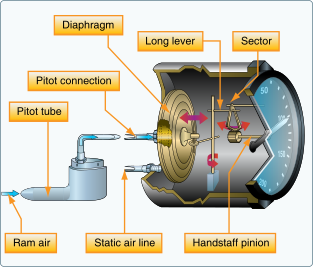
\includegraphics[width=0.5\textwidth]{01-EtudeAeronefs/img/instruments/schemaBadin.pdf}
  		\legende{Principe de fonctionnement d'un anémomètre}{img:schemaBadin}
	\end{figure}	
	
	\paragraph{Le tube Pitot}
	
	L'anémomètre fonctionne grâce à un capteur appelé \gls{pitot} situé à l'extérieur de l'appareil. Sur les avions légers, ce capteur est habituellement situé sous l'aile. Sur les avions de ligne, ce capteur est généralement situé sur la partie avant du fuselage. Ces positionnements permettent d'éloigner le Pitot des influences aérodynamiques de surfaces portantes.
	
	Le tube Pitot est une sonde très importante pour le pilotage des aéronefs. C'est pourquoi ce capteur est généralement protégé lorsque l'aéronef est au sol, en mettant dessus un étui communément appelé \textit{flamme}. Lors de la pré-vol, on retire l'étui et on vérifie l'absence d'obstruction. Sur beaucoup d'avions, le tube Pitot peut également être chauffé pour empêcher la formation de glace nuisible à son fonctionnement.
	
	\histoire{Le tube Pitot a été inventé en 1732 par le physicien français Henri Pitot.}
	
	\begin{figure}[H]
	\begin{minipage}[c]{0.5\linewidth}
	\includegraphics[width=\linewidth]{01-EtudeAeronefs/img/tubePitotC172.jpg}
	\legende{Tube Pitot équipé de sa protection sur Cessna 172}{img:tubePitotC172}
	\end{minipage}
	\hfill
	\begin{minipage}[c]{0.5\linewidth}
	\includegraphics[width=\linewidth]{01-EtudeAeronefs/img/tubesPitotG6000.jpg}
	\legende{Tubes Pitot sur Bombardier Global 6000}{img:tubesPitotG6000}
	\end{minipage}
	\end{figure}
	
	\subsubsection{L'altimètre}
	
	L'\gls{altimètre} \anglais{altimeter} est un instrument qui permet de mesurer l'altitude ou la hauteur par rapport à une référence (par exemple le niveau de la mer ou la hauteur de l'aérodrome). Il fonctionne en mesurant la pression atmosphérique. En effet, la pression atmosphérique diminue avec l'altitude. Mesurer cette pression permet donc de mesurer indirectement l'altitude. \\
	
	Les altimètres sont généralement gradués en pieds\footnote{font exception à cette règle : \begin{itemize}
	\item la Russie
	\item les vélivoles (planeurs)
	\end{itemize} qui expriment leurs altitudes et hauteurs en mètres.}.
	
	\begin{figure}[H]	
	\centering
	\begin{tikzpicture}
		\altiHpa{4500}{1015}
	\end{tikzpicture}
	\legende{Un altimètre, calé à 1015~hPa et affichant 4500 pieds}{tikz:instrumentsBase}
	\end{figure}
	
	\paragraph{Lecture de l'altimètre}
	L'altimètre se lit à la façon d'une horloge : l'aiguille longue et fine représente les centaines de pieds, tandis que l'aiguille courte et épaisse représente les milliers de pieds. Sur la plupart des altimètres, une aiguille plus fine permet de décompter les dizaines de milliers de pieds.
	
	\begin{figure}[H]	
	\centering
	\altiHpaAnimChangementAlti{720}{0}{16000}{980}
	\legende{Montée d'une altitude de 0 à 16\,000 pieds}{img:schemaAltimetre}
	\end{figure}
	
	\paragraph{Fonctionnement} La pièce qui effectue la mesure dans un altimètre est la capsule \gls{anéroïde}. Il s'agit d'une capsule métallique étanche et conçue pour pouvoir être déformée par la pression atmosphérique. La mesure de cette déformation est ensuite amplifiée pour être affichée sur le cadran de l'altimètre.
	
	\begin{figure}[H]
  		\centering
    		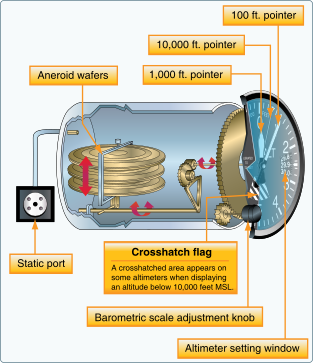
\includegraphics[width=0.5\textwidth]{01-EtudeAeronefs/img/instruments/schemaAltimetre.pdf}
  		\legende{Principe de fonctionnement d'un altimètre}{img:schemaAltimetre}
	\end{figure}	
	
	\paragraph{Calage altimétrique}
	On a vu que l'altimètre mesure l'altitude en mesurant une pression. A une altitude donnée, la valeur de cette pression varie selon le lieu et le temps.
	
	L'altimètre est donc équipé d'un bouton rotatif qui permet à l'équipage de modifier la pression de référence. Cette référence est affichée dans une petite fenêtre de l'instrument. La pression de référence est soit communiquée par le contrôle aérien, soit déterminée au sol par le pilote à un point de référence (typiquement : altitude de l'aérodrome).
	
	\info{La pression atmosphérique est mesurée en hectopascal (hPa) en Europe et dans la plupart des pays. Elle est mesurée en pouces de mercure (inHg) aux États-Unis d'Amérique (pression moyenne au niveau de la mer : 1013,25~hPa = 29,92~inHg).}
	
	Il existe 3 principales références en altimétrie :
	\begin{itemize}
		\item le \acrshort{qnh}
		\item le \acrshort{qfe}
		\item le calage standard 1013,25~hPa
	\end{itemize}
	
	\astuce{Quand on augmente la valeur du QNH affichée dans la fenêtre de réglage, l'altitude indiquée par l'altimètre augmente. \\ Dans l'exemple ci-dessus, le pilote passe le réglage de 970 à 1035~hPa.\begin{figure}[H]	
	\centering
	\altiAnimReglageQnhHpa{360}{1500}{970}{1035}
	\legende{Effet du réglage du QNH}{img:schemaAltimetre}
	\end{figure}}
	
	\subparagraph{Le calage au QNH}
	Le calage au QNH indique une hauteur par rapport au niveau moyen de la mer. Avec ce calage, lorsque l'avion est au sol, l'altimètre affiche l'altitude du terrain.
	
	C'est ce calage qui est transmis dans les bulletins météo d'aérodrome.
	
	\subparagraph{Le calage au QFE}
	Le calage au QFE permet à l'équipage de connaître sa hauteur par rapport au sol. À ce calage, l'altimètre affiche 0 pieds lorsque l'avion est au sol.
	
	\info{De nos jours, ce calage est très rarement utilisé.}
	
	\subparagraph{Le calage à la pression standard}
	Ce calage est utilisé exclusivement en vol au delà d'une altitude dite de transition (TA, en France généralement 5000~pieds). Pour passer au calage standard, on affiche 1013.25 hPa (la pression moyenne au  niveau de la mer) dans la fenêtre de pression de l'altimètre. Dans ce cas, l'altimètre affichera un niveau de vol \anglais{flight level} (FL), qui correspond à l'altitude en centaines de pieds (FL55 = 5500~pieds).
	
	\subsubsection{Le variomètre}
	Le \gls{variomètre} \anglais{variometer} est un instrument qui indique la vitesse verticale (montée/descente) d'un aéronef. Cette vitesse est exprimée en pieds/minutes (ft/min)\footnote{Sauf en planeur et en Russie, qui utilisent le mètre/minute}.
	
	\begin{figure}[H]	
	\centering
	\begin{tikzpicture}
		\vario{-500}
	\end{tikzpicture}
	\legende{Un variomètre affichant -500 ft/min}{tikz:instrumentsBase}
	\end{figure}
	
	Le variomètre mesure les variations de pression atmosphériques. Pour cela, il est équipé d'une capsule analogue à celle que l'on trouve dans un altimètre. Cette capsule est reliée à la sonde de pression statique. Cet ensemble est scellé dans un compartiment équipé d'un dispositif de fuite calibré. 
	
	\begin{figure}[H]
  		\centering
    		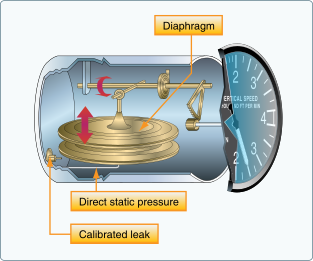
\includegraphics[width=0.5\textwidth]{01-EtudeAeronefs/img/instruments/schemaVario.pdf}
  		\legende{Principe de fonctionnement d'un variomètre}{img:schemaVario}
	\end{figure}	
	
	Quand l'altitude de l'aéronef varie, la pression statique fait varier l'épaisseur de la capsule. Cette variation met en mouvement l'aiguille qui indique le taux de montée/descente. Comme l'instrument est équipé d'un dispositif de fuite calibrée, la pression dans l'instrument (et donc autour de la capsule) a tendance à revenir à l'équilibre avec la pression statique. Tant que la variation d'altitude (et donc de pression statique) est maintenue, l'aiguille du variomètre indiquera à une valeur différente de 0. Si la variation d'altitude s'arrête, la pression dans l'instrument finira pas redevenir égale à la pression statique (grâce à la fuite calibrée), ce qui remettra l'indication à 0.
	
	\info{Le variomètre ne peut afficher une vitesse réellement instantanée : il y a un léger délais entre la variation de vitesse verticale et son affichage sur le variomètre.}
	
	\subsubsection{L'horizon artificiel}
	L'\gls{horizon artificiel} \anglais{attitude indicator} est un appareil qui affiche l'inclinaison et l'assiette d'un aéronef. L'horizon artificiel permet de piloter l'aéronef lorsqu'il évolue sans visibilité, dans un nuage, par exemple.
	
%\begin{table}[H]
%  \centering
%  \begin{tabular}{c c}
%    \begin{minipage}{.45\textwidth}
%      \begin{figure}[H]
%  		\centering
%  		\begin{tikzpicture}
%			\horizon{0}{0}
%		\end{tikzpicture}
%		\legende{Un horizon artificiel}{tikz:instrumentsBase}		
%		\end{figure}
%    \end{minipage}
%    &
%    \begin{minipage}{.55\textwidth}
%      \begin{figure}[H]
%  		\centering
%    		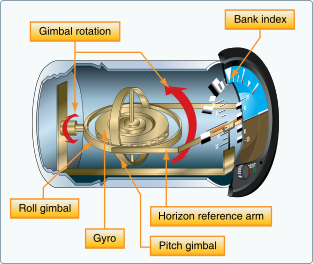
\includegraphics[width=1.0\textwidth]{01-EtudeAeronefs/img/instruments/schemaHorizon.pdf}
%  		\legende{Principe de fonctionnement d'un horizon artificiel}{img:schemaHorizon}
%	  \end{figure}
%    \end{minipage} 
%  \end{tabular}
%  %\caption{}
%\end{table}
	
	\begin{figure}[H]	
	\centering
	\begin{tikzpicture}
		\horizon{0}{0}
	\end{tikzpicture}
	\legende{Un horizon artificiel}{tikz:instrumentsBase}
	\end{figure}
	
	\begin{figure}[H]
  		\centering
    		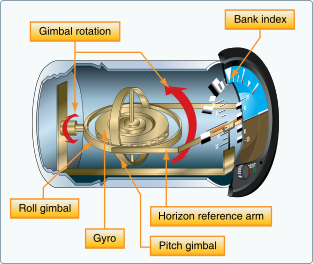
\includegraphics[width=0.5\textwidth]{01-EtudeAeronefs/img/instruments/schemaHorizon.pdf}
  		\legende{Principe de fonctionnement d'un horizon artificiel}{img:schemaHorizon}
	\end{figure}
	
		\paragraph{Lecture de l'horizon artificiel}
		Sur l'horizon artificiel, la maquette qui représente l'avion est fixe :
		\begin{figure}[H]
  		\centering
    		\includegraphics[width=0.2\textwidth]{01-EtudeAeronefs/img/instruments/ai/maquette.pdf}
  		\legende{Maquette de l'avion sur l'horizon artificiel}{img:instrumentsBase}
		\end{figure}
		
		
\begin{table}[H]
  \centering
  \begin{tabular}{c c}
    \begin{minipage}{.49\textwidth}
      \begin{figure}[H]
  		\centering
  		\begin{tikzpicture}
		\horizon{0}{10}
		\end{tikzpicture}
  				\legende{Assiette de montée, 10°}{tikz:instrumentsBase}		
		\end{figure}
    \end{minipage}
    &
    \begin{minipage}{.49\textwidth}
      \begin{figure}[H]
  		\centering
  		\begin{tikzpicture}
		\horizon{0}{-10}
		\end{tikzpicture}
  				\legende{Assiette de descente, -10°}{tikz:instrumentsBase}			
		\end{figure}
    \end{minipage} 
  \end{tabular}
  %\caption{}
\end{table}

\begin{table}[H]
  \centering
  \begin{tabular}{c c}
    \begin{minipage}{.49\textwidth}
      \begin{figure}[H]
  		\centering
  		\begin{tikzpicture}
		\horizon{-30}{0}
		\end{tikzpicture}
  				\legende{Inclinaison à gauche, 30°}{tikz:instrumentsBase}			
		\end{figure}
    \end{minipage} 
    &
    \begin{minipage}{.49\textwidth}
      \begin{figure}[H]
  		\centering
  		\begin{tikzpicture}
		\horizon{30}{0}
		\end{tikzpicture}
  				\legende{Inclinaison à droite, 30°}{tikz:instrumentsBase}		
		\end{figure}
    \end{minipage}
  \end{tabular}
  %\caption{}
\end{table}
	
	\subsubsection{L'indicateur de virage}\label{chap:etudeAer:indicateurVirage}
	L'\gls{indicateur de virage} \anglais{turn coordinator}, également appelé bille-aiguille, est un instrument qui permet de visualiser l'inclinaison d'un aéronef ainsi que de contrôler le dérapage (lacet).
	
	La fonction d'indication d'inclinaison est complémentaire de celle de l'horizon artificiel et peut-être utilisée cas de défaillance de l'horizon.
	
	\begin{figure}[H]	
	\centering
	\begin{tikzpicture}
		\indicateurVirage{0}{0}
	\end{tikzpicture}
	\legende{Un indicateur de virage}{tikz:instrumentsBase}
	\end{figure}
	
	\info{Cet appareil affiche en réalité un taux de virage. Lorsque la maquette de l'avion est alignée avec l'un des 2 repères du pourtour de l'instrument, l'aéronef effectue un tour complet (360°) en 2 minutes. Ce taux est appelée "taux standard".}
	
	\subsection{Les instruments de navigation}
	\subsubsection{Le compas magnétique}	
	Le \gls{compas magnétique} \anglais{magnetic compass}, également appelé \gls{boussole} utilise le champ magnétique terrestre pour fournir un cap à l'équipage.
	
	\begin{figure}[H]
  	\centering
    \includegraphics[width=0.4\textwidth]{01-EtudeAeronefs/img/compas.jpg}
  	\legende{Un compas magnétique}{img:compas}
	\end{figure}	
	
	\subsubsection{Le conservateur de cap}
	
	Le \gls{conservateur de cap} \anglais{heading indicator}, également appelé directionnel, est un instrument gyroscopique qui permet d'afficher le cap suivi par l'aéronef. Il s'utilise en complément de la boussole et offre un confort d'usage supérieur à celle-ci. En effet, la boussole peut devenir difficilement lisible en cas de turbulences ou de vibrations, car son indication sera instable. On recale le conservateur de cap sur boussole dans les phases de vol stables.
	
	\begin{figure}[H]	
	\centering
	\begin{tikzpicture}
		\conservateurCap{85}
	\end{tikzpicture}
	\legende{Un conservateur de cap indiquant un cap à 85°}{tikz:instrumentsBase}
	\end{figure}
	
	\subsubsection{Les instruments de radionavigation}
	\info{L'utilisation pratique des instruments de navigation sera abordée dans le chapitre dédié à la navigation. Ces instruments ne seront donc que brièvement décrits ici.}
	
	\paragraph{Le VOR et le DME}
	Le \acrshort{vor} (\anglais{\acrlong{vor}} et le \acrshort{dme} (\anglais{\acrlong{dme}}
	
	\paragraph{L'ILS}
	L\acrshort{ils} \anglais{\acrlong{ils}}
	
	\begin{figure}[H]	
	\centering
	\begin{tikzpicture}
		\ils{qdm=95, ecartLoc=0.3, ecartGlide=0.6, afficherFlagNav=false}
	\end{tikzpicture}
	\legende{Un ILS}{tikz:instrumentsBase}
	\end{figure}
	
	\paragraph{L'ADF}
	L'\acrshort{adf} \anglais{\acrlong{adf}}
	
	\subsection{Les instruments de contrôle de la machine}
	
		\subsubsection{Compte-tours}
		Le compte-tours \anglais{tachymeter} ou tachymètre permet de connaître le régime de rotation du moteur. Sur beaucoup d'avions, l'hélice est en prise directe sur le moteur, donc cet indicateur indique également la vitesse de rotation de l'hélice.
	
		\begin{figure}[H]
  			\centering
    			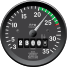
\includegraphics[width=0.4\textwidth]{01-EtudeAeronefs/img/instruments/compteTour.pdf}
  			\legende{Un compte-tours moteur}{img:compteTour}
		\end{figure}	
		
		Sur monomoteur léger, le compte-tours est souvent le seul moyen de vérification et de réglage de la puissance délivrée par le moteur. Il permet de vérifier que la totalité de la puissance est disponible au décollage, mais également d'afficher une puissance donnée (par exemple $2400~tr/min$ pour $75~\%$ de la puissance.
		
		\subsubsection{Pression d'admission}
		\begin{figure}[H]
  			\centering
    			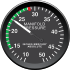
\includegraphics[width=0.4\textwidth]{01-EtudeAeronefs/img/instruments/pressionDAdmission.pdf}
  			\legende{Pression d'admission}{img:pressionDAdmission}
		\end{figure}	
		
		\subsubsection{Débit carburant, EGT}
		\begin{figure}[H]
  			\centering
    			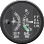
\includegraphics[width=0.4\textwidth]{01-EtudeAeronefs/img/instruments/egtFueFlow.pdf}
  			\legende{Débit de carburant et température des gaz d'échappement}{img:egtFueFlow}
		\end{figure}	
		
		\subsubsection{Jauges de carburant}
		\begin{figure}[H]
  			\centering
    			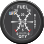
\includegraphics[width=0.4\textwidth]{01-EtudeAeronefs/img/instruments/jaugeCarburant.pdf}
  			\legende{Jauges de carburant}{img:jaugeCarburant}
		\end{figure}	
		
		\subsubsection{Température et pression d'huile}
		Ces indicateurs sont parmi les plus importants pour surveiller le moteur. En effet, un moteur qui fonctionne sans pression d'huile sera très rapidement détruit. L'indicateur de pression d'huile est systématiquement vérifié immédiatement après la mise en route, et une absence de montée de la pression d'huile aboutis toujours à l'arrêt immédiat du moteur pour éviter son endommagement.
		
		L'indicateur de pression d'huile permet de vérifier que la température d'huile est comprise dans la plage idéale, avant le décollage mais aussi pendant tout le vol.
		\begin{figure}[H]
  			\centering
    			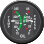
\includegraphics[width=0.4\textwidth]{01-EtudeAeronefs/img/instruments/temperaturePressionHuile.pdf}
  			\legende{Indicateur de température et de pressiond d'huile}{img:temperaturePressionHuile}
		\end{figure}	
		
		\subsubsection{Génération électrique}
		\begin{figure}[H]
  			\centering
    			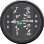
\includegraphics[width=0.4\textwidth]{01-EtudeAeronefs/img/instruments/voltmetreAmperemetre.pdf}
  			\legende{Voltmètre et ampèremètre}{img:voltmetreAmperemetre}
		\end{figure}	
	
	\subsection{Conception des planches de bord}
	Il n'existe pas de normalisation des la disposition des instruments dans un cockpit. Cependant, on retrouve dans la majorité des cockpits une disposition standard "en T" des instruments de navigation de base : anémomètre, horizon artificiel et altimètre sur une ligne, et conservateur de cap sous l'horizon artificiel.
	
	\begin{figure}[H]	
	\centering
	\resizebox{0.5\width}{0.5\height}{
		\dessinerTdB{vitesse=120, 
		altitude=4500,
		calageAltitude=1013,
		vz = -300,
		cap = 180,
		assiette = -12,
		inclinaison = 23,
		derapage = 0.5,
    		virage = 0.75,
		afficherT=true}
	}
	\legende{Disposition typique d'une planche de bord}{tikz:plancheDeBord}
	\end{figure}
	
	Cette disposition type est issue de l'expérience et permet au pilote d'avoir un circuit visuel confortable dans toutes les phases de vol.
	
	\begin{figure}[H]
	\centering
	\includegraphics[width=0.75\linewidth]{01-EtudeAeronefs/img/DR400plancheDeBord.jpg}
	\legende{Planche de bord d'un DR400}{img:DR400plancheDeBord}
	\end{figure}
	
	\subsection{Le glass cockpit}
	
	De plus en plus d'avions sont équipés d'avionique dite "\gls{glasscockpit}". Ce type d'avionique vise à regrouper l'ensemble des instrument sur un ou plusieurs écrans qui occupent alors la majeure partie de l'espace de la planche de bord.
	
	\begin{figure}[H]
	\begin{minipage}[c]{0.5\linewidth}
	\includegraphics[width=\linewidth]{01-EtudeAeronefs/img/A350Cockpit.jpg}
	\legende{Airbus A350}{img:A350Cockpit}
	\end{minipage}
	\hfill
	\begin{minipage}[c]{0.5\linewidth}
	\includegraphics[width=\linewidth]{01-EtudeAeronefs/img/C172glassCockpit.jpg}
	\legende{Cessna 172 glass cockpit}{img:C172glassCockpit}
	\end{minipage}
	\end{figure}
	
	On retrouve donc sur un affichage synthétique et unifié de l'ensemble des instruments classiques.
	
	\begin{figure}[H]
	\centering
	\includegraphics[width=0.8\linewidth, trim={0 0 0 2.75cm}, clip]{01-EtudeAeronefs/img/G1000-PFD.png}
	\legende{Écran de navigation primaire Garmin G1000}{screenshot:G1000-PFD}
	\end{figure}
	
	\begin{figure}[H]
	\centering
	\includegraphics[width=0.8\linewidth, trim={0 0 0 2.75cm}, clip]{01-EtudeAeronefs/img/G1000-MFD.png}
	\legende{Écran multifonction Garmin G1000}{screenshot:G1000-MFD}
	\end{figure}
	
	\info{Les systèmes \gls{glasscockpit} sont désignés par l'acronyme \acrshort{efis} (système d'instruments de vol électronique \anglais{\acrlong{efis}}). Le pilote doit disposer de la qualification EFIS pour piloter un avion glass cockpit.}